\chapter{Graph Algorithms}
\label{chapter-graphs}

Graphs are ubiquitous in modern society:\ examples encountered by
almost everyone on a daily basis include the hyperlink structure of
the web (simply known as the web graph), social networks (manifest in
the flow of email, phone call patterns, connections on social
networking sites, etc.), and transportation networks (roads, bus
routes, flights, etc.).  Our very own existence is dependent on an
intricate metabolic and regulatory network, which can be characterized
as a large, complex graph involving interactions between genes,
proteins, and other cellular products.  This chapter focuses on graph
algorithms in MapReduce.  Although most of the content has nothing to
do with text processing \emph{per se}, documents frequently exist in
the context of some underlying network, making graph analysis an
important component of many text processing applications.  Perhaps the
best known example is PageRank, a measure of web page quality based on
the structure of hyperlinks, which is used in ranking results for web
search.  As one of the first applications of MapReduce, PageRank
exemplifies a large class of graph algorithms that can be concisely
captured in the programming model.  We will discuss PageRank in detail
later this chapter.

In general, graphs can be characterized by nodes (or vertices) and
links (or edges) that connect pairs of nodes.\footnote{Throughout this
  chapter, we use \emph{node} interchangeably with \emph{vertex} and
  similarly with \emph{link} and \emph{edge}.}  These connections can be
directed or undirected.  In some graphs, there may be an edge from a
node to itself, resulting in a self loop; in others, such edges are
disallowed.  We assume that both nodes and links may be annotated with
additional metadata:\ as a simple example, in a social network where
nodes represent individuals, there might be demographic information
(e.g., age, gender, location) attached to the nodes and type
information attached to the links (e.g., indicating type of
relationship such as ``friend'' or ``spouse'').

Mathematicians have always been fascinated with graphs, dating back to
Euler's paper on the \emph{Seven Bridges of K\"{o}nigsberg} in 1736.
Over the past few centuries, graphs have been extensively studied, and
today much is known about their properties.  Far more than theoretical
curiosities, theorems and algorithms on graphs can be applied to solve
many real-world problems:

\begin{itemize}

\item Graph search and path planning.  Search algorithms on graphs are
  invoked millions of times a day, whenever anyone searches for
  directions on the web.  Similar algorithms are also involved in
  friend recommendations and expert-finding in social networks.  Path
  planning problems involving everything from network packets to
  delivery trucks represent another large class of graph search
  problems.

\item Graph clustering.  Can a large graph be divided into components
  that are relatively disjoint (for example, as measured by
  inter-component links~\cite{Girvan02})?  Among other applications,
  this task is useful for identifying communities in social networks
  (of interest to sociologists who wish to understand how human
  relationships form and evolve) and for partitioning large graphs (of
  interest to computer scientists who seek to better parallelize graph
  processing).  See~\cite{XuR_Wunsch_2005b} for a survey.

\item Minimum spanning trees.  A minimum spanning tree for a graph $G$
  with weighted edges is a tree that contains all vertices of the
  graph and a subset of edges that minimizes the sum of edge weights.
  A real-world example of this problem is a telecommunications company
  that wishes to lay optical fiber to span a number of destinations at
  the lowest possible cost (where weights denote costs).  This
  approach has also been applied to wide variety of problems,
  including social networks and the migration of Polynesian
  islanders~\cite{Hage_1996}.

\item Bipartite graph matching.  A bipartite graph is one whose
  vertices can be divided into two disjoint sets.  Matching problems
  on such graphs can be used to model job seekers looking for
  employment or singles looking for dates.

\item Maximum flow. In a weighted directed graph with two special
  nodes called the source and the sink, the max flow problem involves
  computing the amount of ``traffic'' that can be sent from source to
  sink given various flow capacities defined by edge weights.
  Transportation companies (airlines, shipping, etc.) and network
  operators grapple with complex versions of these problems on a daily
  basis.

\item Identifying ``special'' nodes.  There are many ways to define
  what special means, including metrics based on node in-degree,
  average distance to other nodes, and relationship to cluster
  structure.  These special nodes are important to investigators
  attempting to break up terrorist cells, epidemiologists modeling the
  spread of diseases, advertisers trying to promote products, and many
  others.

\end{itemize}

\noindent A common feature of these problems is the scale of the
datasets on which the algorithms must operate:\ for example, the
hyperlink structure of the web, which contains billions of pages, or
social networks that contain hundreds of millions of individuals.
Clearly, algorithms that run on a single machine and depend on the
entire graph residing in memory are not scalable.  We'd like to put
MapReduce to work on these challenges.\footnote{As a side note, Google
  recently published a short description of a system called
  Pregel~\cite{Malewicz_etal_2009}, based on Valiant's Bulk
  Synchronous Parallel model~\cite{Valiant_CACM1990}, for large-scale
  graph algorithms; a longer description is anticipated in a
  forthcoming paper~\cite{Malewicz_etal_SIGMOD2010}}

This chapter is organized as follows:\ we begin in
Section~\ref{chapter-graphs:graph-representations} with an
introduction to graph representations, and then explore two classic
graph algorithms in MapReduce:\ parallel breadth-first search
(Section~\ref{chapter-graphs:BFS}) and PageRank
(Section~\ref{chapter-graphs:PageRank}).  Before concluding with a
summary and pointing out additional readings,
Section~\ref{chapter-graphs:issues} discusses a number of general
issue that affect graph processing with MapReduce.

\section{Graph Representations}
\label{chapter-graphs:graph-representations}

One common way to represent graphs is with an adjacency matrix.  A
graph with $n$ nodes can be represented as an $n \times n$ square
matrix $M$, where a value in cell $m_{ij}$ indicates an edge from node
$n_i$ to node $n_j$.  In the case of graphs with weighted edges, the
matrix cells contain edge weights; otherwise, each cell contains
either a one (indicating an edge), or a zero (indicating none).  With
undirected graphs, only half the matrix is used (e.g., cells above the
diagonal).  For graphs that allow self loops (a directed edge from a
node to itself), the diagonal might be populated; otherwise, the
diagonal remains empty.
Figure~\ref{figure:chapter-graphs:graph-representations} provides an example
of a simple directed graph (left) and its adjacency matrix
representation (middle).

\begin{figure}[t]
\begin{center}
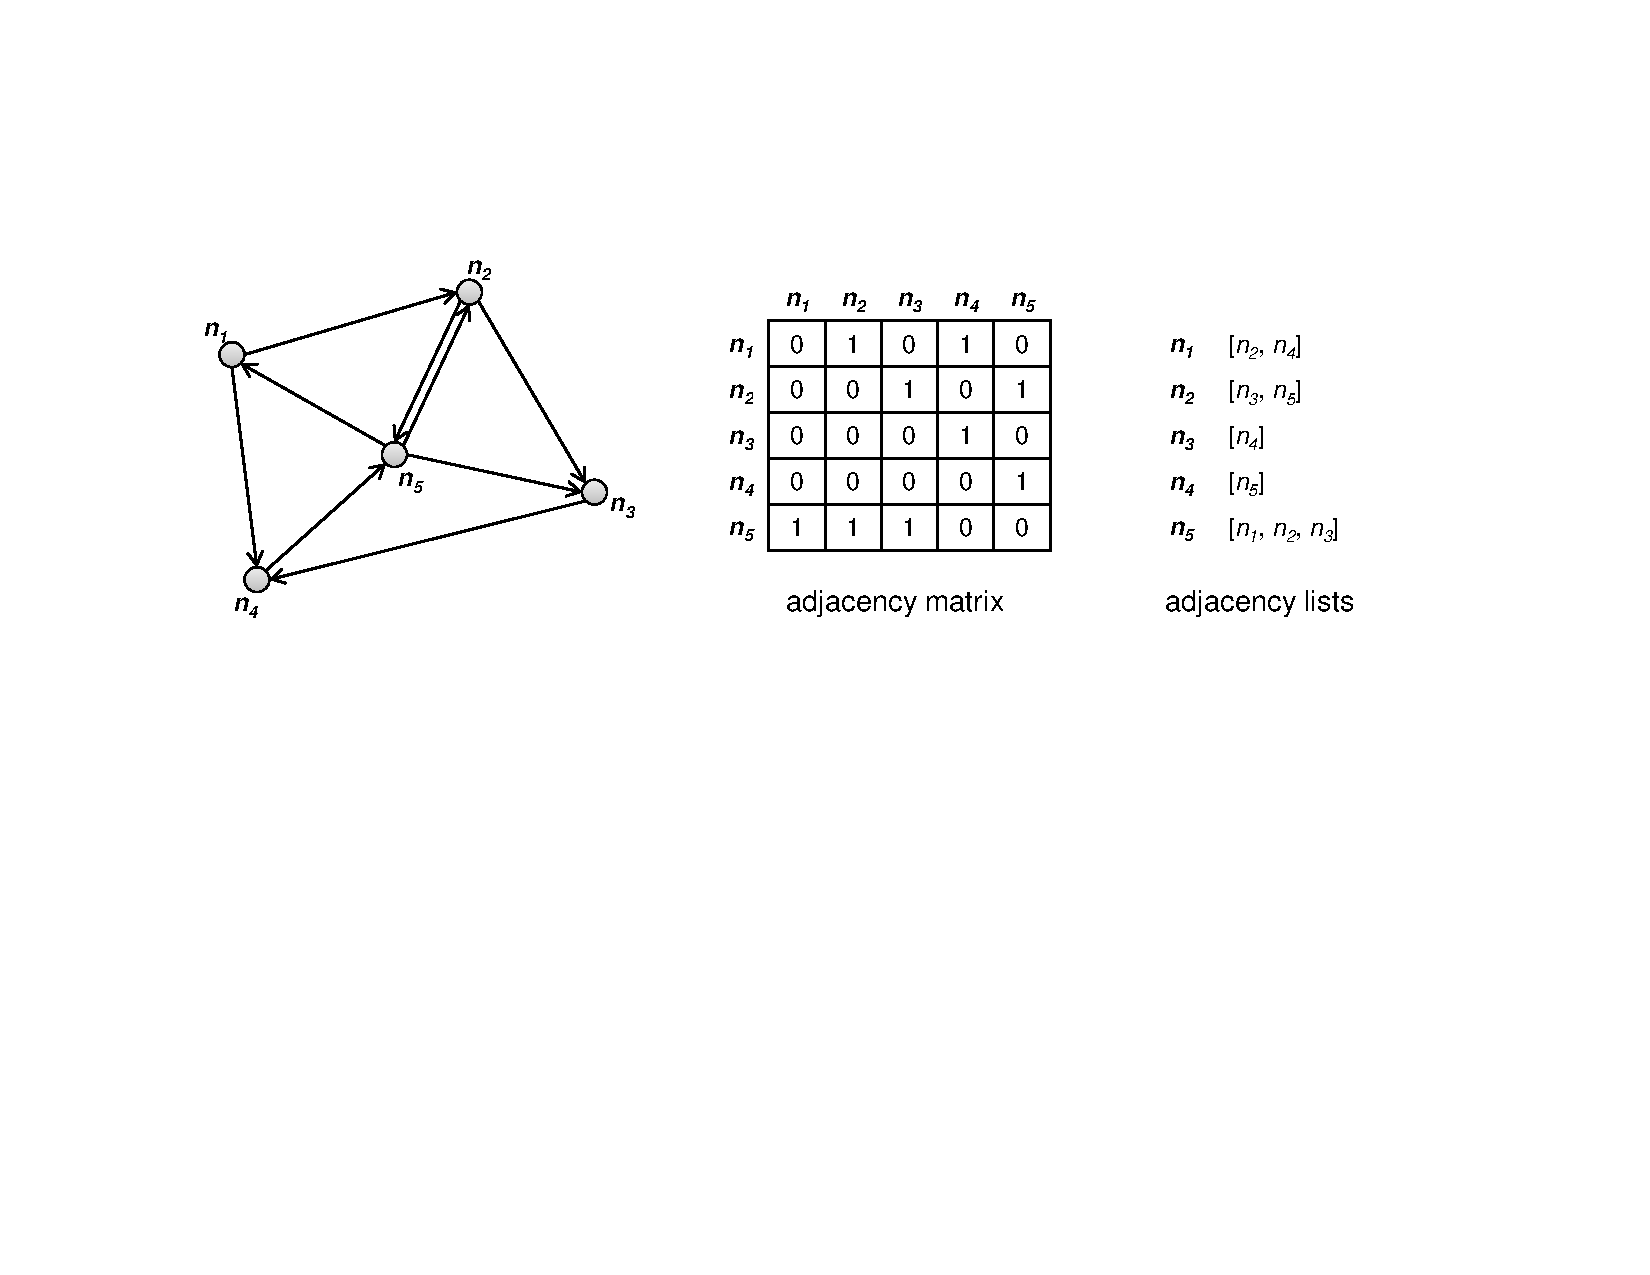
\includegraphics[scale=0.6]{figures/fig-ch5-graph-representations.pdf}
\end{center}
\caption{A simple directed graph (left) represented as an adjacency
  matrix (middle) and with adjacency lists (right).}
\label{figure:chapter-graphs:graph-representations}
\end{figure}

Although mathematicians prefer the adjacency matrix representation of
graphs for easy manipulation with linear algebra, such a
representation is far from ideal for computer scientists concerned
with efficient algorithmic implementations.  Most of the applications
discussed in the chapter introduction involve \emph{sparse} graphs,
where the number of \emph{actual} edges is far smaller than the number
of \emph{possible} edges.\footnote{Unfortunately, there is no precise
  definition of sparseness agreed upon by all, but one common
  definition is that a sparse graph has $O(n)$ edges, where $n$ is the
  number of vertices.}  For example, in a social network of $n$
individuals, there are $n (n-1)$ possible ``friendships'' (where $n$
may be on the order of hundreds of millions).  However, even the most
gregarious will have relatively few friends compared to the size of
the network (thousands, perhaps, but still far smaller than hundreds
of millions).  The same is true for the hyperlink structure of the
web:\ each individual web page links to a minuscule portion of all the
pages on the web.  In this chapter, we assume processing of sparse
graphs, although we will return to this issue in
Section~\ref{chapter-graphs:issues}.

The major problem with an adjacency matrix representation for sparse
graphs is its $O(n^2)$ space requirement.  Furthermore, most of the
cells are zero, by definition.  As a result, most computational
implementations of graph algorithms operate over adjacency lists, in
which a node is associated with neighbors that can be reached via
outgoing edges.
Figure~\ref{figure:chapter-graphs:graph-representations} also shows
the adjacency list representation of the graph under consideration (on
the right).  For example, since $n_1$ is connected by directed edges
to $n_2$ and $n_4$, those two nodes will be on the adjacency list of
$n_1$.  There are two options for encoding undirected graphs:\ one
could simply encode each edge twice (if $n_i$ and $n_j$ are connected,
each appears on each other's adjacency list).  Alternatively, one
could order the nodes (arbitrarily or otherwise) and encode edges only
on the adjacency list of the node that comes first in the ordering
(i.e., if $i<j$, then $n_j$ is on the adjacency list of $n_i$, but not
the other way around).

Note that certain graph operations are easier on adjacency matrices
than on adjacency lists.  In the first, operations on incoming links
for each node translate into a column scan on the matrix, whereas
operations on outgoing links for each node translate into a row scan.
With adjacency lists, it is natural to operate on outgoing links, but
computing anything that requires knowledge of the incoming links of a
node is difficult.  However, as we shall see, the shuffle and sort
mechanism in MapReduce provides an easy way to group edges by their
destination nodes, thus allowing us to compute over incoming edges
with in the reducer.  This property of the execution framework can
also be used to invert the edges of a directed graph, by mapping over
the nodes' adjacency lists and emitting key--value pairs with the
destination node id as the key and the source node id as the
value.\footnote{This technique is used in \emph{anchor text inversion},
  where one gathers the anchor text of hyperlinks pointing to a
  particular page.  It is common practice to enrich a web page's
  standard textual representation with all of the anchor text
  associated with its incoming hyperlinks
  (e.g.,~\cite{Metzler_etal_2009}).}

\section{Parallel Breadth-First Search}
\label{chapter-graphs:BFS}

One of the most common and well-studied problems in graph theory is
the \emph{single-source shortest path} problem, where the task is to
find shortest paths from a source node to all other nodes in the graph
(or alternatively, edges can be associated with costs or weights, in
which case the task is to compute lowest-cost or lowest-weight paths).
Such problems are a staple in undergraduate algorithm courses, where
students are taught the solution using Dijkstra's algorithm.  However,
this famous algorithm assumes sequential processing---how would we
solve this problem in parallel, and more specifically, with MapReduce?

As a refresher and also to serve as a point of comparison, Dijkstra's
algorithm is shown in Algorithm~\ref{algorithm:chapter-graphs:Dijkstra},
adapted from Cormen, Leiserson, and Rivest's classic algorithms
textbook~\cite{CLR} (often simply known as \emph{CLR}).  The input to
the algorithm is a directed, connected graph $G=(V,E)$ represented
with adjacency lists, $w$ containing edge distances such that $w(u,v)
\geq 0$, and the source node $s$.  The algorithm begins by first
setting distances to all vertices $d[v], v \in V$ to $\infty$, except
for the source node, whose distance to itself is zero.  The algorithm
maintains $Q$, a global priority queue of vertices with priorities equal to
their distance values $d$.

\begin{algorithm}[t]
\caption{Dijkstra's algorithm}
\label{algorithm:chapter-graphs:Dijkstra}
Dijkstra's algorithm is based on maintaining a global priority queue
of nodes with priorities equal to their distances from the source
node.  At each iteration, the algorithm expands the node with the
shortest distance and updates distances to all reachable nodes.

  \algrenewcommand\algorithmicfunction{}
  \begin{algorithmic}[1]
    \Function{Dijkstra}{$G, w, s$}
    \State $d[s] \gets 0$
    \ForAll{$\textrm{vertex }v \in V$}
      \State $d[v] \gets \infty$
    \EndFor
    \State $Q \gets \{V\}$
    \While{$Q \ne \emptyset$}
      \State $u \gets \textsc{ExtractMin}(Q)$
      \ForAll{$\textrm{vertex }v \in u.\textsc{AdjacencyList}$}
        \If{$d[v] > d[u] + w(u,v)$}
          \State $d[v] \gets d[u] + w(u,v)$
        \EndIf
      \EndFor
    \EndWhile
    \EndFunction
  \end{algorithmic}
\end{algorithm}

Dijkstra's algorithm operates by iteratively selecting the node with
the lowest current distance from the priority queue (initially, this
is the source node).  At each iteration, the algorithm ``expands''
that node by traversing the adjacency list of the selected node to see
if any of those nodes can be reached with a path of a shorter
distance.  The algorithm terminates when the priority queue $Q$ is
empty, or equivalently, when all nodes have been considered.  Note
that the algorithm as presented in
Algorithm~\ref{algorithm:chapter-graphs:Dijkstra} only computes the shortest
distances.  The actual paths can be recovered by storing
``backpointers'' for every node indicating a fragment of the shortest
path.

\begin{figure}[t]
\begin{center}
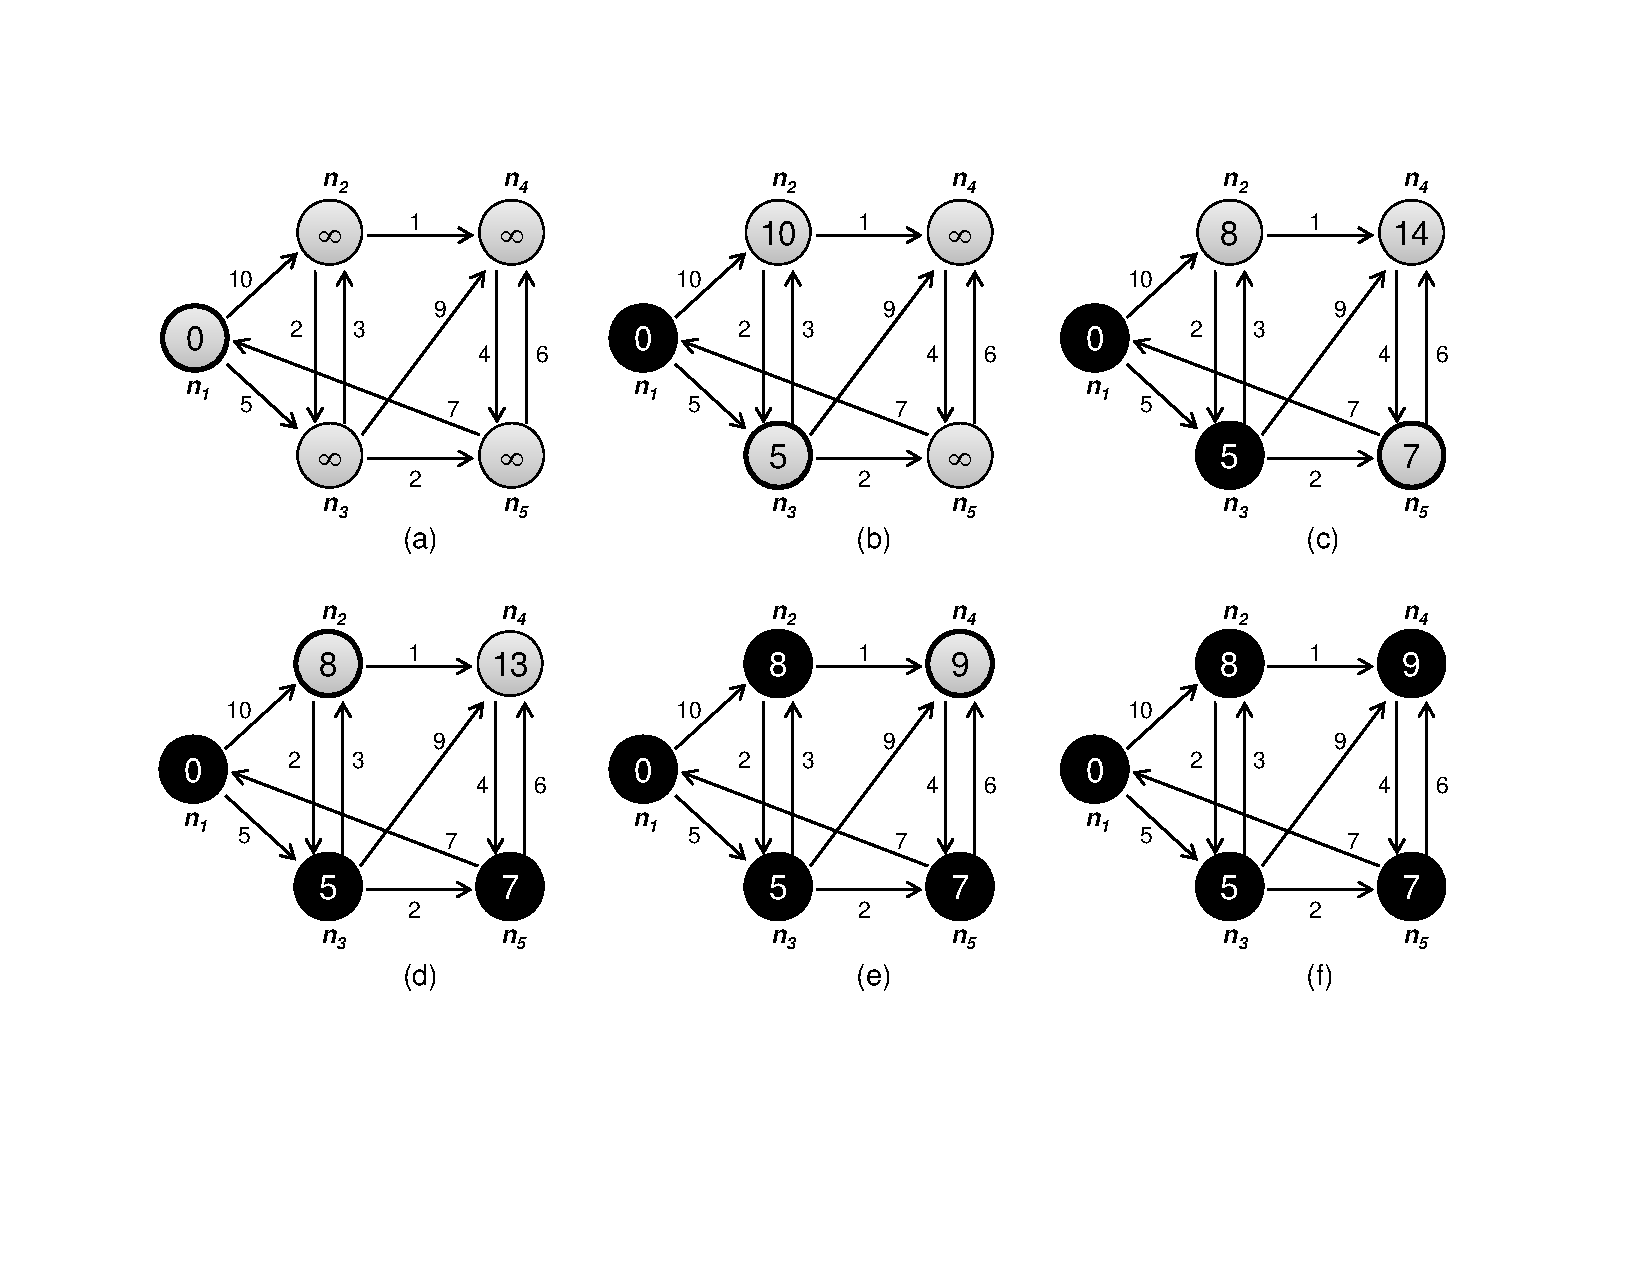
\includegraphics[scale=0.50]{figures/fig-ch5-Dijkstra-example.pdf}
\end{center}
\caption{Example of Dijkstra's algorithm applied to a simple graph
  with five nodes, with $n_1$ as the source and edge distances as
  indicated.  Parts (a)--(e) show the running of the algorithm at each
  iteration, with the current distance inside the node.  Nodes with
  thicker borders are those being expanded; nodes that have already
  been expanded are shown in black.}
\label{figure:chapter-graphs:Dijkstra-example}
\end{figure}

A sample trace of the algorithm running on a simple graph is shown in
Figure~\ref{figure:chapter-graphs:Dijkstra-example} (example also adapted
from \emph{CLR}).  We start out in (a) with $n_1$ having a
distance of zero (since it's the source) and all other nodes having a
distance of $\infty$.  In the first iteration (a), $n_1$ is selected
as the node to expand (indicated by the thicker border).  After the
expansion, we see in (b) that $n_2$ and $n_3$ can be reached at a
distance of 10 and 5, respectively.  Also, we see in (b) that $n_3$ is
the next node selected for expansion.  Nodes we have already
considered for expansion are shown in black.  Expanding $n_3$, we see
in (c) that the distance to $n_2$ has decreased because we've found a
shorter path.  The nodes that will be expanded next, in order, are
$n_5$, $n_2$, and $n_4$.  The algorithm terminates with the end state
shown in (f), where we've discovered the shortest distance to all
nodes.

The key to Dijkstra's algorithm is the priority queue that maintains a
globally-sorted list of nodes by current distance.  This is not
possible in MapReduce, as the programming model does not provide a
mechanism for exchanging global data.  Instead, we adopt a brute force
approach known as parallel breadth-first search.  First, as a
simplification let us assume that all edges have unit distance
(modeling, for example, hyperlinks on the web).  This makes the
algorithm easier to understand, but we'll relax this restriction
later.

The intuition behind the algorithm is this:\ the distance of all nodes
connected directly to the source node is one; the distance of all
nodes directly connected to those is two; and so on.  Imagine water
rippling away from a rock dropped into a pond---that's a good image of
how parallel breadth-first search works.  However, what if there are
multiple paths to the same node?  Suppose we wish to compute the
shortest distance to node $n$.  The shortest path must go through one
of the nodes in $M$ that contains an outgoing edge to $n$:\ we need to
examine all $m \in M$ to find $m_s$, the node with the shortest distance.
The shortest distance to $n$ is the distance to $m_s$ plus one.

Pseudo-code for the implementation of the parallel breadth-first
search algorithm is provided in
Algorithm~\ref{algorithm:chapter-graphs:BFS}.  As with Dijkstra's algorithm,
we assume a connected, directed graph represented as adjacency lists.
Distance to each node is directly stored alongside the adjacency list
of that node, and initialized to $\infty$ for all nodes except for the
source node.  In the pseudo-code, we use $n$ to denote the node id (an
integer) and $N$ to denote the node's corresponding data structure
(adjacency list and current distance).  The algorithm works by mapping
over all nodes and emitting a key-value pair for each neighbor on the
node's adjacency list.  The key contains the node id of the neighbor,
and the value is the current distance to the node plus one.  This
says:\ if we can reach node $n$ with a distance $d$, then we must be
able to reach all the nodes that are connected to $n$ with distance
$d+1$.  After shuffle and sort, reducers will receive keys
corresponding to the destination node ids and distances corresponding
to all paths leading to that node.  The reducer will select the
shortest of these distances and then update the distance in the node
data structure.

\begin{algorithm}[t]
\caption{Parallel breath-first search}
\label{algorithm:chapter-graphs:BFS}
The mappers emit distances to reachable nodes, while the reducers
select the minimum of those distances for each destination node.  Each
iteration (one MapReduce job) of the algorithm expands the ``search
frontier'' by one hop.

\algrenewcommand\algorithmicfunction{\textbf{class}}
\algrenewcommand\algorithmicprocedure{\textbf{method}}
  \begin{algorithmic}[1]
    \Function{Mapper}{}
    \Procedure{Map}{$\textrm{nid }n, \textrm{node }N$}
    \State $d \gets N.\textsc{Distance}$
    \State $\textsc{Emit}(\textrm{nid }n, N)$\Comment{Pass along graph structure}
    \ForAll{$\textrm{nodeid }m \in N.\textsc{AdjacencyList}$}
      \State $\textsc{Emit}(\textrm{nid }m, d+1)$\Comment{Emit distances to reachable nodes}
    \EndFor
    \EndProcedure
    \EndFunction
  \end{algorithmic}

  \begin{algorithmic}[1]
    \Function{Reducer}{}
    \Procedure{Reduce}{$\textrm{nid }m, [d_1, d_2, \ldots ]$}
    \State $d_{min} \gets \infty$
    \State $M \gets \emptyset$
    \ForAll{$d \in \textrm{counts }[d_1, d_2, \ldots ]$}
      \If{$\textsc{IsNode}(d)$}
        \State $M \gets d$\Comment{Recover graph structure}
      \ElsIf{$d < d_{min}$}\Comment{Look for shorter distance}
        \State $d_{min} \gets d$
      \EndIf
    \EndFor
    \State $M.\textsc{Distance} \gets d_{min}$\Comment{Update shortest distance}
    \State $\textsc{Emit}(\textrm{nid }m, \textrm{node }M)$
    \EndProcedure
    \EndFunction
  \end{algorithmic}
\end{algorithm}

It is apparent that parallel breadth-first search is an iterative
algorithm, where each iteration corresponds to a MapReduce job.  The
first time we run the algorithm, we ``discover'' all nodes that are
connected to the source.  The second iteration, we discover all nodes
connected to those, and so on.  Each iteration of the algorithm
expands the ``search frontier'' by one hop, and, eventually, all nodes
will be discovered with their shortest distances (assuming a
fully-connected graph).  Before we discuss termination of the
algorithm, there is one more detail required to make the parallel
breadth-first search algorithm work.  We need to ``pass along'' the
graph structure from one iteration to the next.  This is accomplished
by emitting the node data structure itself, with the node id as a key
(Algorithm~\ref{algorithm:chapter-graphs:BFS}, line 4 in the mapper).  In the
reducer, we must distinguish the node data structure from distance
values (Algorithm~\ref{algorithm:chapter-graphs:BFS}, lines 5--6 in the reducer),
and update the minimum distance in the node data structure before
emitting it as the final value.  The final output is now ready to
serve as input to the next iteration.\footnote{Note that in this
  algorithm we are overloading the value type, which can either be a
  distance (integer) or a complex data structure representing a node.
  The best way to achieve this in Hadoop is to create a wrapper object
  with an indicator variable specifying what the content is.}

So how many iterations are necessary to compute the shortest distance
to all nodes?  The answer is the diameter of the graph, or the
greatest distance between any pair of nodes.  This number is
surprisingly small for many real-world problems:\ the saying ``six
degrees of separation'' suggests that everyone on the planet is
connected to everyone else by at most six steps (the people a person
knows are one step away, people that they know are two steps away,
etc.).  If this is indeed true, then parallel breadth-first search on
the global social network would take at most six MapReduce iterations.
For more serious academic studies of ``small world'' phenomena in
networks, we refer the reader to a number of
publications~\cite{Granovetter73,Granovetter83,Watts_Strogatz_1998,Albert_Barabasi_2002}.
In practical terms, we iterate the algorithm until there are no more
node distances that are $\infty$.  Since the graph is connected, all
nodes are reachable, and since all edge distances are one, all
discovered nodes are guaranteed to have the shortest distances (i.e.,
there is not a shorter path that goes through a node that hasn't been
discovered).

The actual checking of the termination condition must occur outside of
MapReduce.  Typically, execution of an iterative MapReduce algorithm
requires a non-MapReduce ``driver'' program, which submits a MapReduce
job to iterate the algorithm, checks to see if a termination condition
has been met, and if not, repeats.  Hadoop provides a lightweight API
for constructs called ``counters'', which, as the name suggests, can be
used for counting events that occur during execution, e.g., number
of corrupt records, number of times a certain condition is met, or
anything that the programmer desires.  Counters can be defined to
count the number of nodes that have distances of $\infty$:\ at the end
of the job, the driver program can access the final counter value and
check to see if another iteration is necessary.

Finally, as with Dijkstra's algorithm in the form presented earlier,
the parallel breadth-first search algorithm only finds the shortest
distances, not the actual shortest paths.  However, the path can be
straightforwardly recovered.  Storing ``backpointers'' at each node,
as with Dijkstra's algorithm, will work, but may not be efficient
since the graph needs to be traversed again to reconstruct the path
segments.  A simpler approach is to emit paths along with distances in
the mapper, so that each node will have its shortest path easily
accessible at all times.  The additional space requirements for
shuffling these data from mappers to reducers are relatively modest,
since for the most part paths (i.e., sequence of node ids) are relatively short.

\begin{figure}[t]
\begin{center}
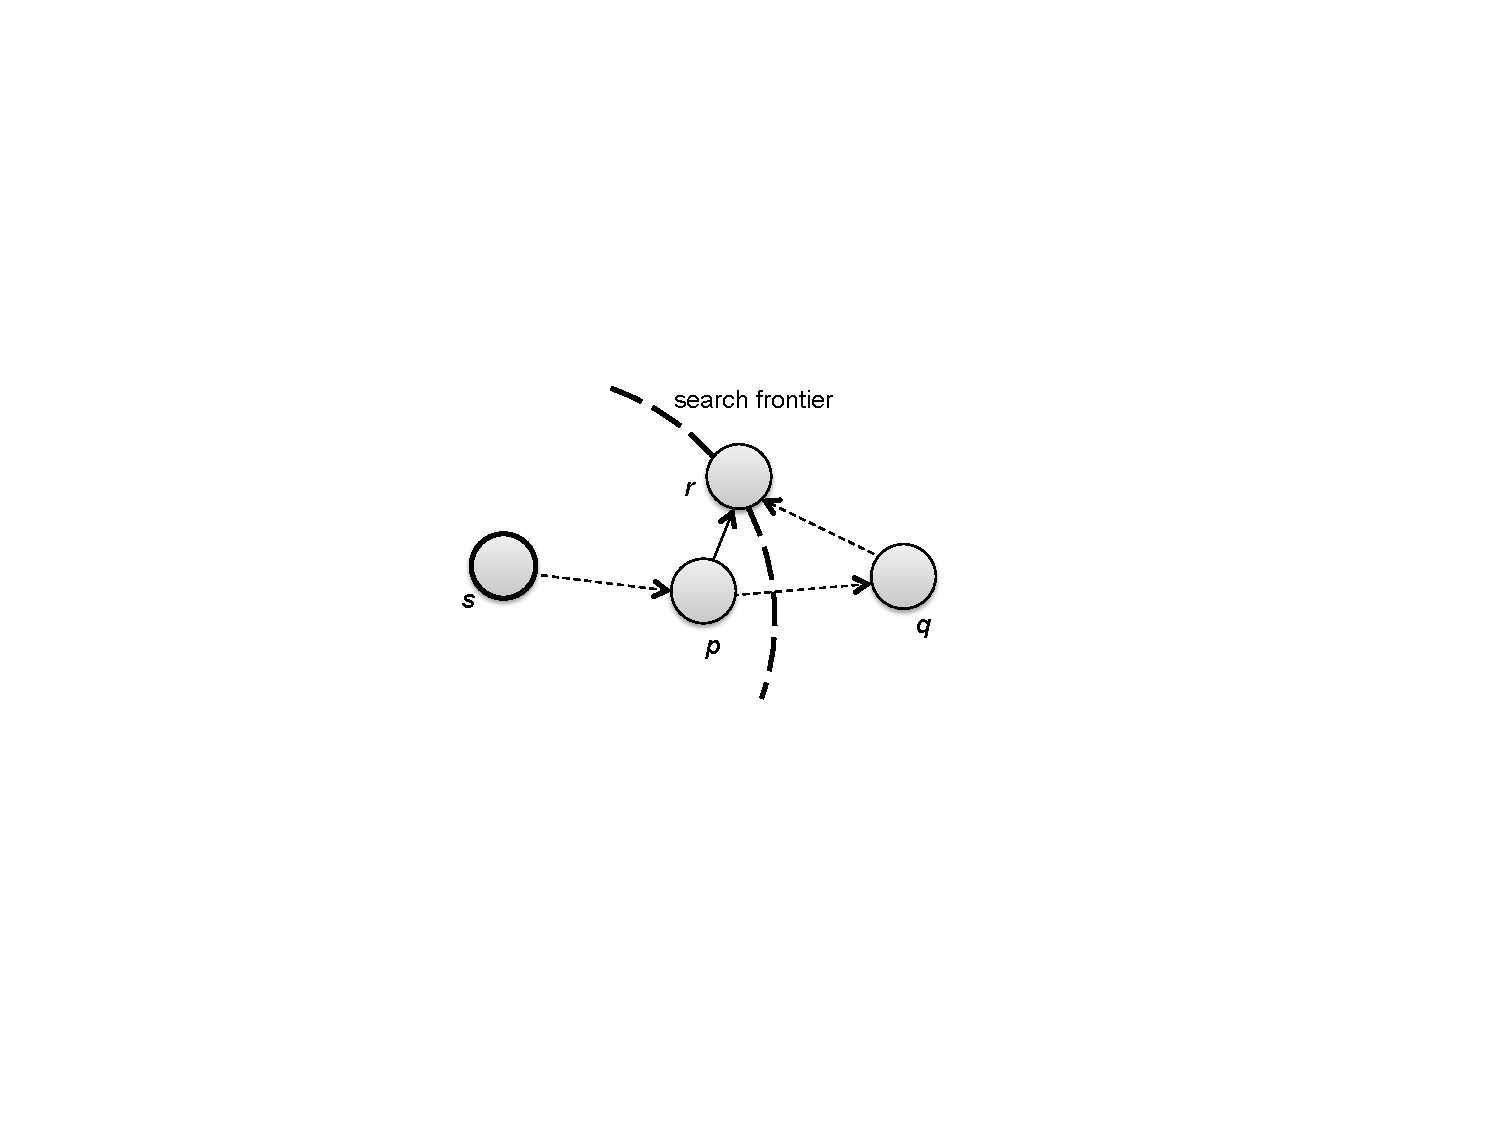
\includegraphics[scale=0.6]{figures/fig-ch5-search-frontier.pdf}
\end{center}
\caption{In the single source shortest path problem with arbitrary
  edge distances, the shortest path from source $s$ to node $r$ may go
  outside the current search frontier, in which case we will not find
  the shortest distance to $r$ until the search frontier expands to
  cover $q$.}
\label{figure:chapter-graphs:search-frontier}
\end{figure}

Up until now, we have been assuming that all edges are unit distance.
Let us relax that restriction and see what changes are required in the
parallel breadth-first search algorithm.  The adjacency lists, which
were previously lists of node ids, must now encode the edge distances
as well.  In line 6 of the mapper code in
Algorithm~\ref{algorithm:chapter-graphs:BFS}, instead of emitting $d+1$ as
the value, we must now emit $d+w$ where $w$ is the edge distance.  No
other changes to the algorithm are required, but the termination
behavior is very different.  To illustrate, consider the graph
fragment in Figure~\ref{figure:chapter-graphs:search-frontier}, where
$s$ is the source node, and in this iteration, we just ``discovered''
node $r$ for the very first time.  Assume for the sake of argument
that we've already discovered the shortest distance to node $p$, and
that the shortest distance to $r$ so far goes through $p$.  This,
however, does not guarantee that we've discovered the shortest
distance to $r$, since there may exist a path going through $q$ that
we haven't encountered yet (because it lies outside the search
frontier).\footnote{Note that the same argument does not apply to the
  unit edge distance case:\ the shortest path cannot lie outside the
  search frontier since any such path would necessarily be longer.}
However, as the search frontier expands, we'll eventually cover $q$
and all other nodes along the path from $p$ to $q$ to $r$---which
means that with sufficient iterations, we will discover the shortest
distance to $r$.  But how do we know that we've found the shortest
distance to $p$?  Well, if the shortest path to $p$ lies within the
search frontier, we would have already discovered it.  And if it
doesn't, the above argument applies.  Similarly, we can repeat the
same argument for all nodes on the path from $s$ to $p$.  The
conclusion is that, with sufficient iterations, we'll eventually
discover all the shortest distances.

\begin{figure}[t]
\begin{center}
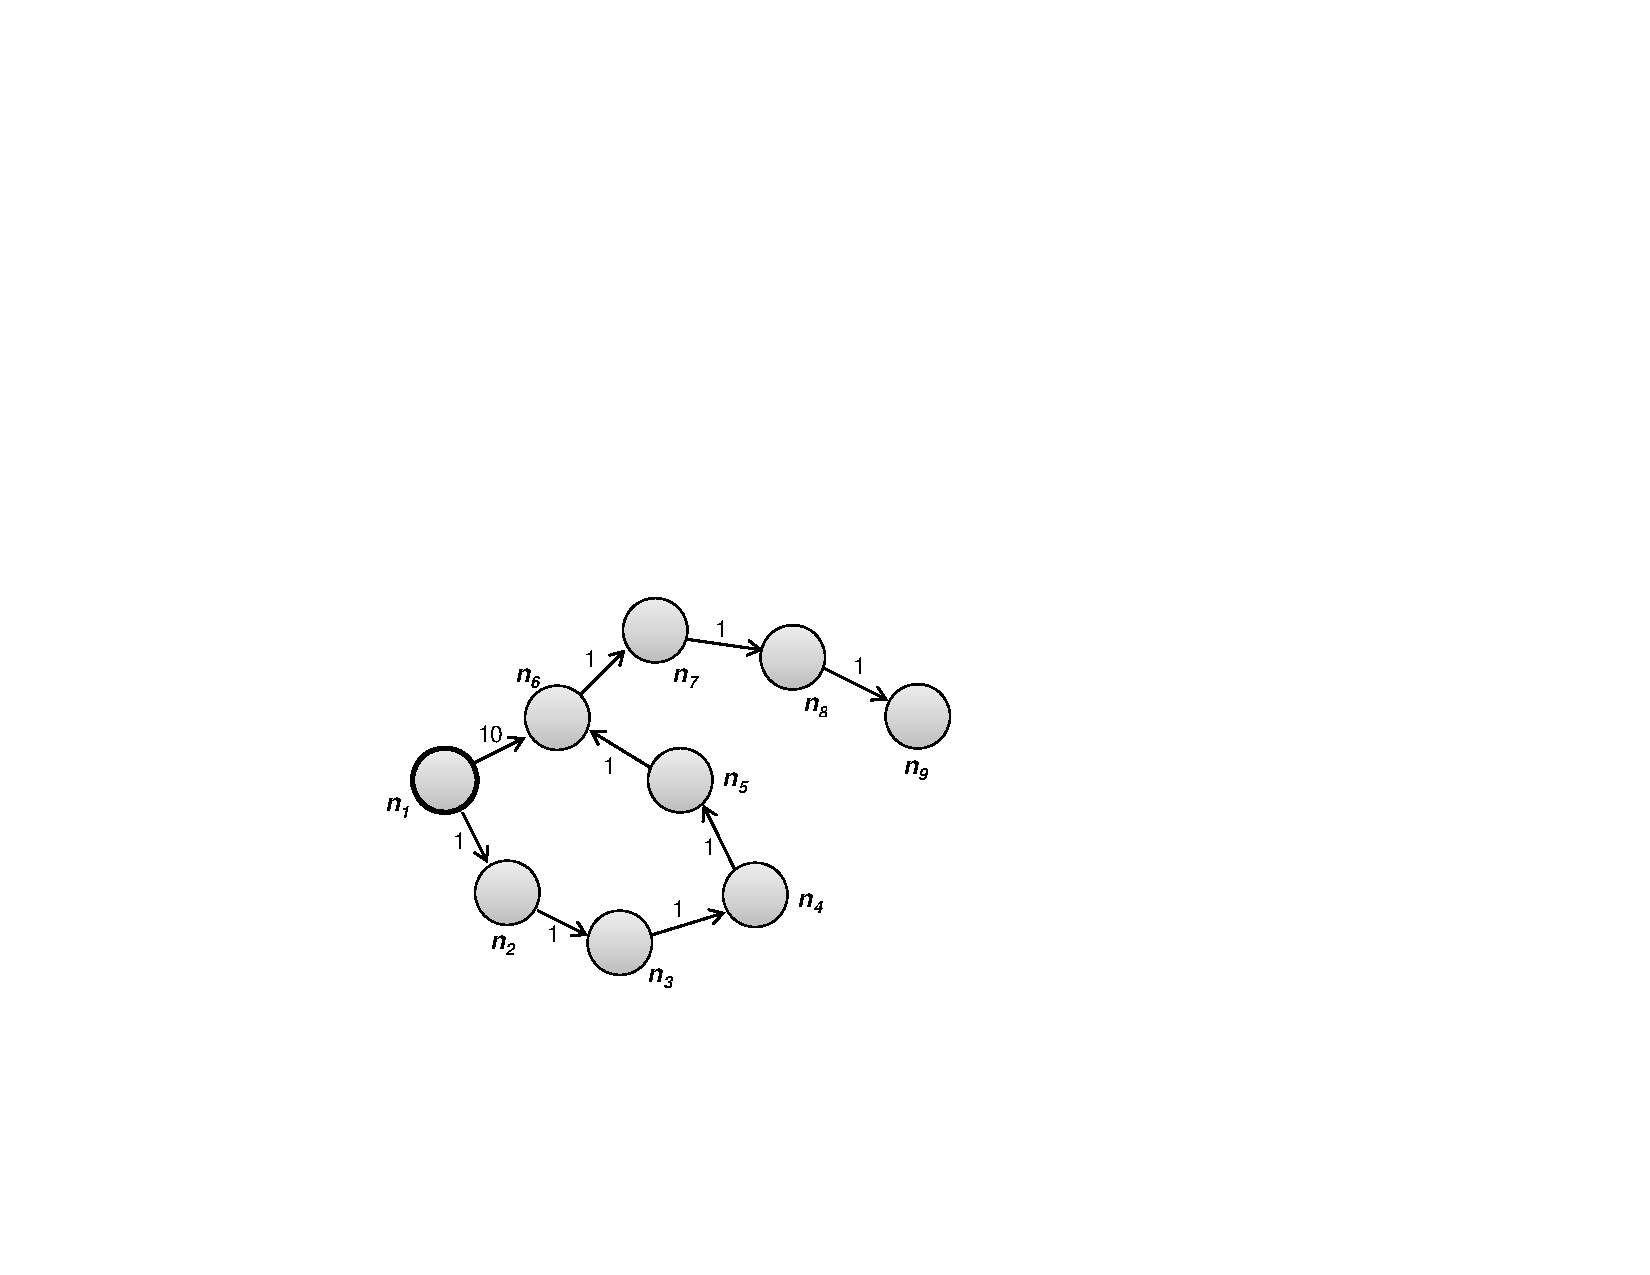
\includegraphics[scale=0.6]{figures/fig-ch5-screwy-graph.pdf}
\end{center}
\caption{A sample graph that elicits worst-case behavior for parallel
  breadth-first search.  Eight iterations are required to discover
  shortest distances to all nodes from $n_1$.}
\label{figure:chapter-graphs:screwy-graph}
\end{figure}

So exactly how many iterations does ``eventually'' mean?  In the worst
case, we might need as many iterations as there are nodes in the graph
minus one.  In fact, it is not difficult to construct graphs that will
elicit this worse-case
behavior:\ Figure~\ref{figure:chapter-graphs:screwy-graph} provides an
example, with $n_1$ as the source.  The parallel breadth-first search
algorithm would not discover that the shortest path from $n_1$ to
$n_6$ goes through $n_3$, $n_4$, and $n_5$ until the fifth iteration.
Three more iterations are necessary to cover the rest of the graph.
Fortunately, for most real-world graphs, such extreme cases are rare,
and the number of iterations necessary to discover all shortest
distances is quite close to the diameter of the graph, as in the unit
edge distance case.

In practical terms, how do we know when to stop iterating in the case
of arbitrary edge distances?  The algorithm can terminate when
shortest distances at every node no longer change.  Once again, we can
use counters to keep track of such events.  Every time we encounter a
shorter distance in the reducer, we increment a counter.  At the end
of each MapReduce iteration, the driver program reads the counter
value and determines if another iteration is necessary.

Compared to Dijkstra's algorithm on a single processor, parallel
breadth-first search in MapReduce can be characterized as a brute
force approach that ``wastes'' a lot of time performing computations
whose results are discarded.  At each iteration, the algorithm
attempts to recompute distances to all nodes, but in reality only
useful work is done along the search frontier:\ inside the search
frontier, the algorithm is simply repeating previous
computations.\footnote{Unless the algorithm discovers an instance of
  the situation described in
  Figure~\ref{figure:chapter-graphs:search-frontier}, in which case,
  updated distances will propagate inside the search frontier.}
Outside the search frontier, the algorithm hasn't discovered any paths
to nodes there yet, so no meaningful work is done.  Dijkstra's
algorithm, on the other hand, is far more efficient.  Every time a
node is explored, we're guaranteed to have already found the shortest
path to it.  However, this is made possible by maintaining a global
data structure (a priority queue) that holds nodes sorted by
distance---this is not possible in MapReduce because the programming
model does not provide support for global data that is mutable and
accessible by the mappers and reducers.  These inefficiencies
represent the cost of parallelization.

The parallel breadth-first search algorithm is instructive in that it
represents the prototypical structure of a large class of graph
algorithms in MapReduce.  They share in the following characteristics:

\begin{itemize}

\item The graph structure is represented with adjacency lists, which is
  part of some larger node data structure that may contain additional
  information (variables to store intermediate output, features of the
  nodes).  In many cases, features are attached to edges as well
  (e.g., edge weights).

\item The MapReduce algorithm maps over the node data structures and
  performs a computation that is a function of features of the node,
  intermediate output attached to each node, and features of the
  adjacency list (outgoing edges and their features).  In other words,
  computations can only involve a node's internal state and its local
  graph structure.  The results of these computations are emitted as
  values, keyed with the node ids of the neighbors (i.e., those nodes
  on the adjacency lists).  Conceptually, we can think of this as
  ``passing'' the results of the computation along outgoing edges.  In
  the reducer, the algorithm receives all partial results that have
  the same destination node, and performs another computation
  (usually, some form of aggregation).

\item In addition to computations, the graph itself is also passed
  from the mapper to the reducer.  In the reducer, the data structure
  corresponding to each node is updated and written back to disk.

\item Graph algorithms in MapReduce are generally iterative, where the
  output of the previous iteration serves as input to the next
  iteration.  The process is controlled by a non-MapReduce driver
  program that checks for termination.

\end{itemize}

\noindent For parallel breadth-first search, the mapper computation is
the current distance plus edge distance (emitting distances to
neighbors), while the reducer computation is the \textsc{Min} function
(selecting the shortest path).  As we will see in the next section,
the MapReduce algorithm for PageRank works in much the same way.

\section{PageRank}
\label{chapter-graphs:PageRank}

PageRank~\cite{Page_etal_1999} is a measure of web page quality based
on the structure of the hyperlink graph.  Although it is only one of
thousands of features that is taken into account in Google's search
algorithm, it is perhaps one of the best known and most studied.

A vivid way to illustrate PageRank is to imagine a random web
surfer:\ the surfer visits a page, randomly clicks a link on that
page, and repeats ad infinitum.  PageRank is a measure of how
frequently a page would be encountered by our tireless web surfer.
More precisely, PageRank is a probability distribution over nodes in
the graph representing the likelihood that a random walk over the link
structure will arrive at a particular node.  Nodes that have high
in-degrees tend to have high PageRank values, as well as nodes that
are linked to by other nodes with high PageRank values.  This behavior
makes intuitive sense:\ if PageRank is a measure of page quality, we
would expect high-quality pages to contain ``endorsements'' from many
other pages in the form of hyperlinks.  Similarly, if a high-quality
page links to another page, then the second page is likely to be high
quality also.  PageRank represents one particular approach to
inferring the quality of a web page based on hyperlink structure; two
other popular algorithms, not covered here, are
SALSA~\cite{Lempel_Moran_TOIS2001} and HITS~\cite{Kleinberg_JACM1999}
(also known as ``hubs and authorities'').

The complete formulation of PageRank includes an additional component.
As it turns out, our web surfer doesn't just randomly click links.
Before the surfer decides where to go next, a biased coin is
flipped---heads, the surfer clicks on a random link on the page as
usual.  Tails, however, the surfer ignores the links on the page and
randomly ``jumps'' or ``teleports'' to a completely different page.

But enough about random web surfing.  Formally, the PageRank $P$ of a
page $n$ is defined as follows:

\begin{equation}
P(n) = \alpha \left( \frac{1}{|G|} \right) + (1-\alpha) \sum_{m \in L(n)} \frac{P(m)}{C(m)}
\end{equation}

\noindent where $|G|$ is the total number of nodes (pages) in the
graph, $\alpha$ is the random jump factor, $L(n)$ is the set of pages
that link to $n$, and $C(m)$ is the out-degree of node $m$ (the number
of links on page $m$).  The random jump factor $\alpha$ is sometimes
called the ``teleportation'' factor; alternatively, $(1-\alpha)$ is
referred to as the ``damping'' factor.

Let us break down each component of the formula in detail.  First,
note that PageRank is defined recursively---this gives rise to an
iterative algorithm we will detail in a bit.  A web page $n$ receives
PageRank ``contributions'' from all pages that link to it, $L(n)$.
Let us consider a page $m$ from the set of pages $L(n)$:\ a random
surfer at $m$ will arrive at $n$ with probability $1/C(m)$ since a
link is selected at random from all outgoing links.  Since the PageRank
value of $m$ is the probability that the random surfer will be at $m$,
the probability of arriving at $n$ from $m$ is $P(m)/C(m)$.  To
compute the PageRank of $n$, we need to sum contributions from all
pages that link to $n$.  This is the summation in the second half of
the equation.  However, we also need to take into account the random
jump:\ there is a $1/|G|$ chance of landing at any particular page,
where $|G|$ is the number of nodes in the graph.  Of course, the two
contributions need to be combined:\ with probability $\alpha$ the
random surfer executes a random jump, and with probability $1-\alpha$
the random surfer follows a hyperlink.

Note that PageRank assumes a community of honest users who are not
trying to ``game'' the measure.  This is, of course, not true in the
real world, where an adversarial relationship exists between search
engine companies and a host of other organizations and individuals
(marketers, spammers, activists, etc.) who are trying to manipulate
search results---to promote a cause, product, or service, or in some
cases, to trap and intentionally deceive users (see, for
example,~\cite{Baeza-Yates_etal_2005,Garcia-Molina_etal_2005}).  A
simple example is a so-called ``spider trap'', a infinite chain of
pages (e.g., generated by CGI) that all link to a single page (thereby
artificially inflating its PageRank).  For this reason, PageRank is
only one of thousands of features used in ranking web pages.

The fact that PageRank is recursively defined 
translates into an iterative algorithm which is quite similar in basic
structure to parallel breadth-first search.  We start by presenting an
informal sketch.  At the beginning of each iteration, a node passes its
PageRank contributions to other nodes that it is connected to.  Since
PageRank is a probability distribution, we can think of this as
spreading probability mass to neighbors via outgoing links.  To
conclude the iteration, each node sums up all PageRank contributions
that have been passed to it and computes an updated PageRank score.
We can think of this as gathering probability mass passed to a node
via its incoming links.  This algorithm iterates until PageRank values
don't change anymore.

\begin{figure}[t]
\begin{center}
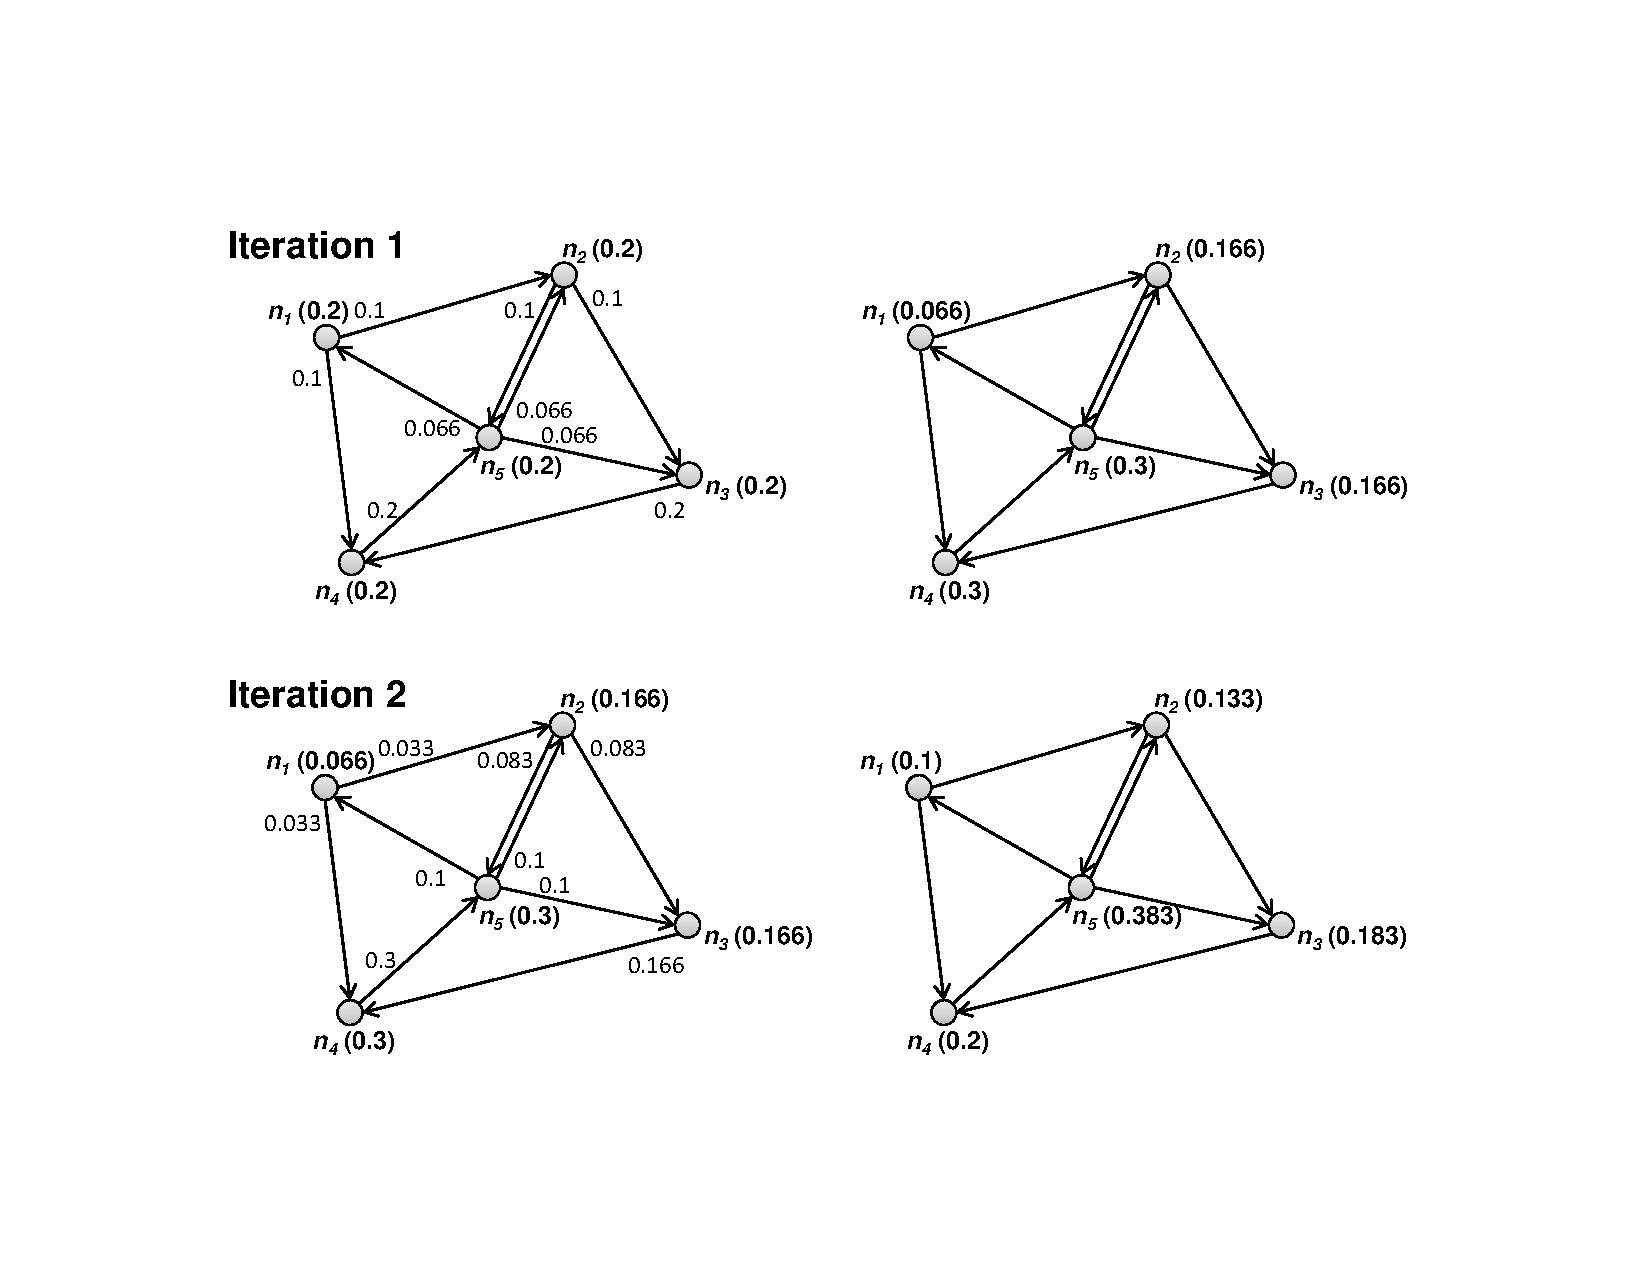
\includegraphics[scale=0.6]{figures/fig-ch5-PageRank-toy-example.pdf}
\end{center}
\caption{PageRank toy example showing two iterations, top and bottom.
  Left graphs show PageRank values at the beginning of each iteration
  and how much PageRank mass is passed to each neighbor.  Right graphs
  show updated PageRank values at the end of each iteration.}
\label{figure:chapter-graphs:PageRank-toy}
\end{figure}

Figure~\ref{figure:chapter-graphs:PageRank-toy} shows a toy example that
illustrates two iterations of the algorithm.  As a simplification, we
ignore the random jump factor for now (i.e., $\alpha=0$) and further
assume that there are no dangling nodes (i.e., nodes with no outgoing
edges).  The algorithm begins by initializing a uniform distribution
of PageRank values across nodes.  In the beginning of the first
iteration (top, left), partial PageRank contributions are sent from
each node to its neighbors connected via outgoing links.  For example,
$n_1$ sends $0.1$ PageRank mass to $n_2$ and $0.1$ PageRank mass to
$n_4$.  This makes sense in terms of the random surfer model:\ if the
surfer is at $n_1$ with a probability of $0.2$, then the surfer could end up
either in $n_2$ or $n_4$ with a probability of $0.1$ each.  The same
occurs for all the other nodes in the graph:\ note that $n_5$ must
split its PageRank mass three ways, since it has three neighbors, and
$n_4$ receives all the mass belonging to $n_3$ because $n_3$ isn't
connected to any other node.  The end of the first iteration is shown
in the top right:\ each node sums up PageRank contributions from its
neighbors.  Note that since $n_1$ has only one incoming link, from
$n_3$, its updated PageRank value is smaller than before, i.e., it
``passed along'' more PageRank mass than it received.  The exact same
process repeats, and the second iteration in our toy example is
illustrated by the bottom two graphs.  At the beginning of each
iteration, the PageRank values of all nodes sum to one.  PageRank mass
is preserved by the algorithm, guaranteeing that we continue to have a
valid probability distribution at the end of each iteration.

Pseudo-code of the MapReduce PageRank algorithm is shown in
Algorithm~\ref{algorithm:chapter-graphs:PageRank}; it is simplified in that we
continue to ignore the random jump factor and assume no dangling nodes
(complications that we will return to later).  An illustration of the
running algorithm is shown in
Figure~\ref{figure:chapter-graphs:PageRank-MapReduce-example} for the first
iteration of the toy graph in
Figure~\ref{figure:chapter-graphs:PageRank-toy}.  The algorithm maps over
the nodes, and for each node computes how much PageRank mass needs to
be distributed to its neighbors (i.e., nodes on the adjacency list).
Each piece of the PageRank mass is emitted as the value, keyed by the node
ids of the neighbors.  Conceptually, we can think of this as passing
PageRank mass along outgoing edges.

\begin{algorithm}[t]
 \caption{PageRank (simplified)}
\label{algorithm:chapter-graphs:PageRank}
In the map phase we evenly divide up each node's PageRank mass and
pass each piece along outgoing edges to neighbors.  In the reduce
phase PageRank contributions are summed up at each destination node.
Each MapReduce job corresponds to one iteration of the algorithm. This
algorithm does not handle dangling nodes and the random jump factor.

\algrenewcommand\algorithmicfunction{\textbf{class}}
\algrenewcommand\algorithmicprocedure{\textbf{method}}
  \begin{algorithmic}[1]
    \Function{Mapper}{}
    \Procedure{Map}{$\textrm{nid }n, \textrm{node }N$}
    \State $p \gets N.\textsc{PageRank} / |N.\textsc{AdjacencyList}|$
    \State $\textsc{Emit}(\textrm{nid }n, N)$\Comment{Pass along graph structure}
    \ForAll{$\textrm{nodeid }m \in N.\textsc{AdjacencyList}$}
      \State $\textsc{Emit}(\textrm{nid }m, p)$\Comment{Pass PageRank mass to neighbors}
    \EndFor
    \EndProcedure
    \EndFunction
  \end{algorithmic}

  \begin{algorithmic}[1]
    \Function{Reducer}{}
    \Procedure{Reduce}{$\textrm{nid }m, [p_1, p_2, \ldots ]$}
    \State $M \gets \emptyset$
    \ForAll{$p \in \textrm{counts }[p_1, p_2, \ldots ]$}
      \If{$\textsc{IsNode}(p)$}
        \State $M \gets p$\Comment{Recover graph structure}
      \Else
        \State $s \gets s + p$\Comment{Sum incoming PageRank contributions}
      \EndIf
    \EndFor
    \State $M.\textsc{PageRank} \gets s$
    \State $\textsc{Emit}(\textrm{nid }m, \textrm{node }M)$
    \EndProcedure
    \EndFunction
  \end{algorithmic}
\end{algorithm}

\begin{figure}[t]
\begin{center}
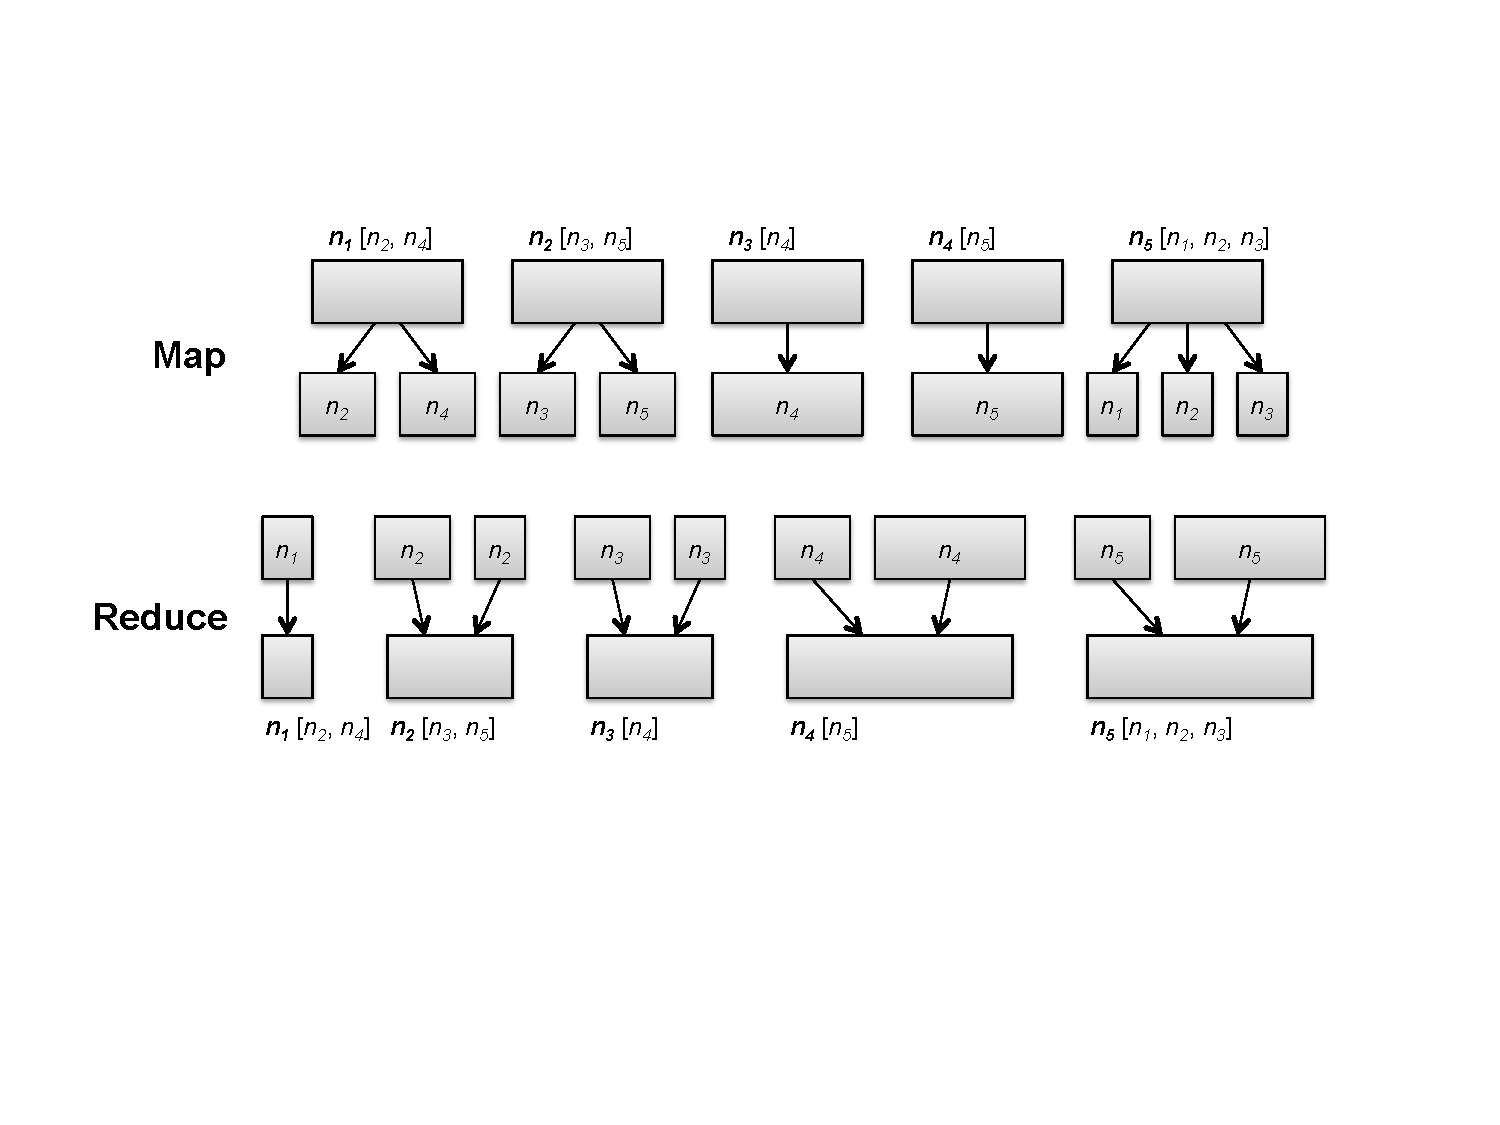
\includegraphics[scale=0.55]{figures/fig-ch5-MapReduce-example.pdf}
\end{center}
\caption{Illustration of the MapReduce PageRank algorithm
  corresponding to the first iteration in
  Figure~\ref{figure:chapter-graphs:PageRank-toy}.  The size of each
  box is proportion to its PageRank value.  During the map phase,
  PageRank mass is distributed evenly to nodes on each node's
  adjacency list (shown at the very top).  Intermediate values are
  keyed by node (shown inside the boxes).  In the reduce phase, all
  partial PageRank contributions are summed together to arrive at
  updated values.}
\label{figure:chapter-graphs:PageRank-MapReduce-example}
\end{figure}

In the shuffle and sort phase, the MapReduce execution framework
groups values (piece of PageRank mass) passed along the graph edges by
destination node (i.e., all edges that point to the same node).  In
the reducer, PageRank mass contributions from all incoming edges are
summed to arrive at the updated PageRank value for each node.  As with
the parallel breadth-first search algorithm, the graph structure
itself must be passed from iteration to iteration.  Each node data
structure is emitted in the mapper and written back out to disk in the
reducer.  All PageRank mass emitted by the mappers are accounted for
in the reducer:\ since we begin with the sum of PageRank values across
all nodes equal to one, the sum of all the updated PageRank values
should remain a valid probability distribution.

Having discussed the simplified PageRank algorithm in MapReduce, let
us now take into account the random jump factor and dangling
nodes:\ as it turns out both are treated similarly.  Dangling nodes
are nodes in the graph that have no outgoing edges, i.e., their
adjacency lists are empty.  In the hyperlink graph of the web, these
might correspond to pages in a crawl that have not been downloaded
yet.  If we simply run the algorithm in
Algorithm~\ref{algorithm:chapter-graphs:PageRank} on graphs with dangling nodes,
the total PageRank mass will not be conserved, since no key-value
pairs will be emitted when a dangling node is encountered in the
mappers.

The proper treatment of PageRank mass ``lost'' at the dangling nodes
is to redistribute it across all nodes in the graph evenly
(cf.~\cite{Bianchini_etal_2005}).  There are many ways to determine
the missing PageRank mass.  One simple approach is by instrumenting
the algorithm in Algorithm~\ref{algorithm:chapter-graphs:PageRank} with
counters:\ whenever the mapper processes a node with an empty
adjacency list, it keeps track of the node's PageRank value in the
counter.  At the end of the iteration, we can access the counter to
find out how much PageRank mass was lost at the dangling
nodes.\footnote{In Hadoop, counters are 8-byte integers:\ a simple
  workaround is to multiply PageRank values by a large constant, and
  then cast as an integer.}  Another approach is to reserve a special
key for storing PageRank mass from dangling nodes.  When the mapper
encounters a dangling node, its PageRank mass is emitted with the
special key; the reducer must be modified to contain special logic for
handling the missing PageRank mass.  Yet another approach is to write
out the missing PageRank mass as ``side data'' for each map task
(using the in-mapper combining technique for aggregation); a final
pass in the driver program is needed to sum the mass across all map
tasks.  Either way, we arrive at the amount of PageRank mass lost at
the dangling nodes---this then must be redistribute evenly across all
nodes.

This redistribution process can be accomplished by mapping over all
nodes again.  At the same time, we can take into account the random
jump factor.  For each node, its current PageRank value $p$ is updated
to the final PageRank value $p'$ according to the following formula:

\begin{equation}
p' = \alpha \left( \frac{1}{|G|} \right) + \left( 1-\alpha \right) \left( \frac{m}{|G|} + p \right)
\end{equation}

\noindent where $m$ is the missing PageRank mass, and $|G|$ is the
number of nodes in the entire graph.  We add the PageRank mass from
link traversal ($p$, computed from before) to the share of the lost
PageRank mass that is distributed to each node ($m/|G|$).  Finally, we
take into account the random jump factor:\ with probability $\alpha$
the random surfer arrives via jumping, and with probability $1-\alpha$
the random surfer arrives via incoming links.  Note that this
MapReduce job requires no reducers.

Putting everything together, one iteration of PageRank requires two
MapReduce jobs:\ the first to distribute PageRank mass along graph
edges, and the second to take care of dangling nodes and the random
jump factor.  At end of each iteration, we end up with
exactly the same data structure as the beginning, which is a
requirement for the iterative algorithm to work.  Also, the PageRank
values of all nodes sum up to one, which ensures a valid probability
distribution.

Typically, PageRank is iterated until convergence, i.e., when the
PageRank values of nodes no longer change (within some tolerance, to
take into account, for example, floating point precision errors).
Therefore, at the end of each iteration, the PageRank driver program
must check to see if convergence has been reached.  Alternative
stopping criteria include running a fixed number of iterations (useful
if one wishes to bound algorithm running time) or stopping when the
\emph{ranks} of PageRank values no longer change.  The latter is useful
for some applications that only care about comparing the PageRank of
two arbitrary pages and do not need the actual PageRank values.  Rank
stability is obtained faster than the actual convergence of values.

In absolute terms, how many iterations are necessary for PageRank to
converge?  This is a difficult question to \emph{precisely} answer
since it depends on many factors, but generally, fewer than one might
expect.  In the original PageRank paper~\cite{Page_etal_1999},
convergence on a graph with 322 million edges was reached in 52
iterations (see also Bianchini et al.~\cite{Bianchini_etal_2005} for
additional discussion).  On today's web, the answer is not very
meaningful due to the adversarial nature of web search as previously
discussed---the web is full of spam and populated with sites that are
actively trying to ``game'' PageRank and related hyperlink-based
metrics.  As a result, running PageRank in its unmodified form
presented here would yield unexpected and undesirable results.  Of
course, strategies developed by web search companies to combat link
spam are proprietary (and closely-guarded secrets, for obvious
reasons)---but undoubtedly these algorithmic modifications impact
convergence behavior.  A full discussion of the escalating ``arms
race'' between search engine companies and those that seek to promote
their sites is beyond the scope of this book.\footnote{For the
  interested reader, the proceedings of a workshop series on
  Adversarial Information Retrieval (AIRWeb) provide great starting
  points into the literature.}

\section{Issues with Graph Processing}
\label{chapter-graphs:issues}

The biggest difference between MapReduce graph algorithms and
single-machine graph algorithms is that with the latter, it is usually
possible to maintain global data structures in memory for fast, random
access.  For example, Dijkstra's algorithm uses a global priority
queue that guides the expansion of nodes.  This, of course, is not
possible with MapReduce---the programming model does not provide any
built-in mechanism for communicating global state.  Since the most
natural representation of large sparse graphs is with adjacency lists,
communication can only occur from a node to the nodes it links to, or
to a node from nodes linked to it---in other words, passing
information is only possible within the local graph
structure.\footnote{Of course, it is perfectly reasonable to compute
  derived graph structures in a pre-processing step.  For example, if
  one wishes to propagate information from a node to all nodes that
  are within two links, one could process graph $G$ to derive graph
  $G'$, where there would exist a link from node $n_i$ to $n_j$ if
  $n_j$ was reachable within two link traversals of $n_i$ in the
  original graph $G$.}

This restriction gives rise to the structure of many graph algorithms
in MapReduce:\ local computation is performed on each node, the
results of which are ``passed'' to its neighbors.  With multiple
iterations, convergence on the global graph is possible.  The passing
of partial results along a graph edge is accomplished by the shuffling
and sorting provided by the MapReduce execution framework.  The amount
of intermediate data generated is on the order of the number of edges,
which explains why all the algorithms we have discussed assume sparse
graphs.  For dense graphs, MapReduce running time would be dominated
by copying intermediate data across the network, which in the worst
case is $O(n^2)$ in the number of nodes in the graph.  Since MapReduce
clusters are designed around commodity networks (e.g., gigabit
Ethernet), MapReduce algorithms are often impractical on large, dense
graphs.

Combiners and the in-mapper combining pattern described in
Section~\ref{chapter3:local-aggregation} can be used to decrease the
running time of graph iterations.  It is straightforward to use
combiners for both parallel breadth-first search and PageRank since
\textsc{Min} and sum, used in the two algorithms, respectively, are
both associative and commutative.  However, combiners are only
effective to the extent that there are opportunities for partial
aggregation---unless there are nodes pointed to by multiple nodes
being processed by an individual map task, combiners are not very
useful.  This implies that it would be desirable to partition large
graphs into smaller components where there are many intra-component
links and fewer inter-component links.  This way, we can arrange the
data such that nodes in the same component are handled by the same map
task---thus maximizing opportunities for combiners to perform local
aggregation.

Unfortunately, this sometimes creates a chick-and-egg problem.  It
would be desirable to partition a large graph to facilitate efficient
processing by MapReduce.  But the graph may be so large that we can't
partition it except with MapReduce algorithms!  Fortunately, in many
cases there are simple solutions around this problem in the form of
``cheap'' partitioning heuristics based on reordering the
data~\cite{Mellor-Crummey_etal_2001}.  For example, in a social
network, we might sort nodes representing users by zip code, as
opposed to by last name---based on the observation that friends tend
to live close to each other.  Sorting by an even more cohesive
property such as school would be even better (if available):\ the
probability of any two random students from the same school knowing
each other is much higher than two random students from different
schools.  Another good example is to partition the web graph by the
language of the page (since pages in one language tend to link mostly
to other pages in that language) or by domain name (since inter-domain
links are typically much denser than intra-domain links).  Resorting
records using MapReduce is both easy to do and a relatively cheap operation---however,
whether the efficiencies gained by this crude form of partitioning are
worth the extra time taken in performing the resort is an empirical
question that will depend on the actual graph structure and algorithm.

Finally, there is a practical consideration to keep in mind when
implementing graph algorithms that estimate probability distributions
over nodes (such as PageRank).  For large graphs, the probability of
any particular node is often so small that it underflows standard
floating point representations.  A very common solution to this
problem is to represent probabilities using their logarithms.  When
probabilities are stored as logs, the product of two values is simply
their sum.  However, addition of probabilities is also necessary, for
example, when summing PageRank contribution for a node.  This can be
implemented with reasonable precision as follows:

\begin{displaymath}
 a \oplus b = \left\{
 \begin{array}{ll}
 b + \log  (1 + e^{a - b} ) & a < b \\
 a + \log  (1 + e^{b - a} ) & a \ge b \\
 \end{array} \right.
 \end{displaymath}

\noindent Furthermore, many math libraries include a \texttt{log1p}
function which computes $\log(1+x)$ with higher precision than the
na\"{i}ve implementation would have when $x$ is very small (as is
often the case when working with probabilities).  Its use may further
improve the accuracy of implementations that use log probabilities.

\section{Summary and Additional Readings}

This chapter covers graph algorithms in MapReduce, discussing in
detail parallel breadth-first search and PageRank.  Both are instances
of a large class of iterative algorithms that share the following
characteristics:

\begin{itemize}

\item The graph structure is represented with adjacency lists.

\item Algorithms map over nodes and pass partial results to nodes on
  their adjacency lists.  Partial results are aggregated for each node
  in the reducer.

\item The graph structure itself is passed from the mapper to the
  reducer, such that the output is in the same form as the input.

\item Algorithms are iterative and under the control of a
  non-MapReduce driver program, which checks for termination at the
  end of each iteration.

\end{itemize}

\noindent The MapReduce programming model does not provide a mechanism
to maintain global data structures accessible and mutable by all the
mappers and reducers.\footnote{However, maintaining
  globally-synchronized state may be possible with the assistance of
  other tools (e.g., a distributed database).} One implication of this
is that communication between pairs of arbitrary nodes is difficult to
accomplish.  Instead, information typically propagates along graph
edges---which gives rise to the structure of algorithms discussed
above.

\paragraph{Additional Readings.} 
The ubiquity of large graphs translates into substantial interest in
scalable graph algorithms using MapReduce in industry, academia, and
beyond.  There is, of course, much beyond what has been covered in
this chapter.  For additional material, we refer readers to the
following:\ Kang et al.~\cite{KangU_etal_2008} presented an approach
to estimating the diameter of large graphs using MapReduce and a
library for graph mining~\cite{KangU_etal_2009};
Cohen~\cite{CohenJonathan_2009} discussed a number of algorithms for
processing undirected graphs, with social network analysis in mind;
Rao and Yarowsky~\cite{Rao_Yarowsky_2009} described an implementation
of label propagation, a standard algorithm for semi-supervised machine
learning, on graphs derived from textual data;
Schatz~\cite{Schatz_2010} tackled the problem of DNA sequence
alignment and assembly with graph algorithms in MapReduce.  Finally,
it is easy to forget that parallel graph algorithms have been studied
by computer scientists for several decades, particular in the PRAM
model~\cite{JaJa_1992,Grama_etal_2003}.  It is not clear, however, to
what extent well-known PRAM algorithms translate naturally into the
MapReduce framework.
